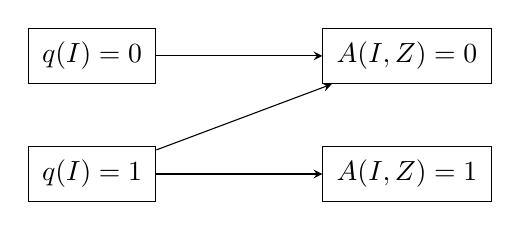
\begin{tikzpicture}[>=stealth]
    % Nodes
    \node[draw, inner sep=5pt] (q0) at (0, 1.5) {$q(I) = 0$};
    \node[draw, inner sep=5pt] (a0) at (4, 1.5) {$A(I, Z) = 0$};
    \node[draw, inner sep=5pt] (q1) at (0, 0)   {$q(I) = 1$};
    \node[draw, inner sep=5pt] (a1) at (4, 0)   {$A(I, Z) = 1$};
    % Arrows connecting the nodes
    \draw[->] (q0) -- (a0);
    \draw[->] (q1) -- (a1);
    \draw[->] (q1) -- (a0);
\end{tikzpicture}